%This figure requires both the shadows and mindmap tikzlibraries. Include them in your header!
\usetikzlibrary{shadows, mindmap}
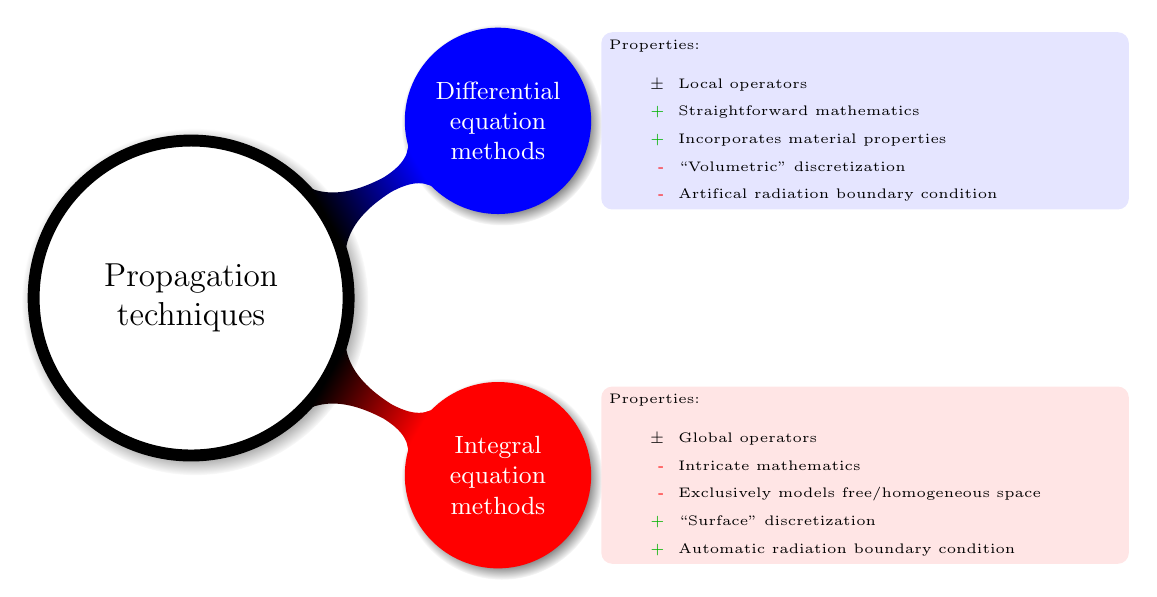
\begin{tikzpicture}[mindmap, >=latex]
  \begin{scope}[
    every node/.style={concept, circular drop shadow,execute at begin node=\hskip0pt},
    root concept/.append style={
      concept color=black, fill=white, line width=1ex, text=black
    },
    text=white,
    IE/.style={concept color=red,faded/.style={concept color=red!50}},
    DE/.style={concept color=blue,faded/.style={concept color=blue!50}},
    measuring complexity/.style={concept color=orange,faded/.style={concept color=orange!50}},
    solving problems/.style={concept color=green!50!black,faded/.style={concept color=green!50!black!50}},
    grow cyclic,
    level 1/.append style={level distance=4.5cm, sibling angle=60},
    level 2/.append style={level distance=3cm,sibling angle=30}]

  \node[root concept]{Propagation techniques}
  child[IE]{ node (IE) {Integral equation methods}}
  child[DE]{ node (DE) {Differential equation methods}};
    \end{scope}
  \begin{scope}[every annotation/.style={fill=blue!10}]
    \node [annotation, xshift=3.5cm, yshift=0.0cm, text width = 6.5cm] at (DE.east) {
      Properties:
       \begin{itemize}
         \setlength\itemsep{0em}
         \item[$\pm$] Local operators
         \item[\textcolor{green!70!black}{+}] Straightforward mathematics
         \item[\textcolor{green!70!black}{+}] Incorporates material properties
         \item[\textcolor{red}{-}] ``Volumetric'' discretization
         \item[\textcolor{red}{-}] Artifical radiation boundary condition
       \end{itemize}
    };
  \end{scope}
  \begin{scope}[every annotation/.style={fill=red!10}]
    \node [annotation, xshift=3.5cm, yshift=-0.0cm, text width = 6.5cm] at (IE.east) {
      Properties:
       \begin{itemize}
         \setlength\itemsep{0em}
         \item[$\pm$] Global operators
         \item[\textcolor{red}{-}] Intricate mathematics
         \item[\textcolor{red}{-}] Exclusively models free/homogeneous space
         \item[\textcolor{green!70!black}{+}] ``Surface'' discretization
         \item[\textcolor{green!70!black}{+}] Automatic radiation boundary condition
       \end{itemize}
    };
  \end{scope}

  %\foreach \x in {10,10.5,...,13}
    %\draw (\x, 1.4) -- (\x, 1.8);

  %\shade [ball color=blue!50] (10, 1.6) circle [radius=0.1cm];
  %\shade [ball color=blue!50] (12.5, 1.6) circle [radius=0.1cm];

  %\draw[->] (10.0, 1.6) to[out=30, in=150] (10.5, 1.6);
  %\draw[->] (10.5, 1.6) to[out=30, in=150] (11.0, 1.6);
  %\draw[->] (11.0, 1.6) to[out=30, in=150] (11.5, 1.6);
  %\draw[->] (11.5, 1.6) to[out=30, in=150] (12.0, 1.6);
  %\draw[->] (12.0, 1.6) to[out=30, in=150] (12.5, 1.6);

  %\node[] at (11.25, 1.2) {\tiny Larger, sparse matrices};
  

  %\draw (10,-1.4) -- (10, -1.8);
  %\draw (12.5,-1.4) -- (12.5, -1.8);

  %\shade [ball color=red!50] (10, -1.6) circle [radius=0.1cm];
  %\shade [ball color=red!50] (12.5, -1.6) circle [radius=0.1cm];

  %\draw[->] (10, -1.6) to[out=30, in=150] (12.5, -1.6);

  %\node[] at (11.25, -2.0) {\tiny Smaller, dense matrices};
\end{tikzpicture}
